\documentclass[]{article}
\usepackage{lmodern}
\usepackage{amssymb,amsmath}
\usepackage{ifxetex,ifluatex}
\usepackage{fixltx2e} % provides \textsubscript
\ifnum 0\ifxetex 1\fi\ifluatex 1\fi=0 % if pdftex
  \usepackage[T1]{fontenc}
  \usepackage[utf8]{inputenc}
\else % if luatex or xelatex
  \ifxetex
    \usepackage{mathspec}
  \else
    \usepackage{fontspec}
  \fi
  \defaultfontfeatures{Ligatures=TeX,Scale=MatchLowercase}
\fi
% use upquote if available, for straight quotes in verbatim environments
\IfFileExists{upquote.sty}{\usepackage{upquote}}{}
% use microtype if available
\IfFileExists{microtype.sty}{%
\usepackage{microtype}
\UseMicrotypeSet[protrusion]{basicmath} % disable protrusion for tt fonts
}{}
\usepackage[margin=1in]{geometry}
\usepackage{hyperref}
\hypersetup{unicode=true,
            pdftitle={Latent Dirichlet Allocation Models Considering Emojis},
            pdfauthor={Taikgun Song},
            pdfborder={0 0 0},
            breaklinks=true}
\urlstyle{same}  % don't use monospace font for urls
\usepackage{longtable,booktabs}
\usepackage{graphicx,grffile}
\makeatletter
\def\maxwidth{\ifdim\Gin@nat@width>\linewidth\linewidth\else\Gin@nat@width\fi}
\def\maxheight{\ifdim\Gin@nat@height>\textheight\textheight\else\Gin@nat@height\fi}
\makeatother
% Scale images if necessary, so that they will not overflow the page
% margins by default, and it is still possible to overwrite the defaults
% using explicit options in \includegraphics[width, height, ...]{}
\setkeys{Gin}{width=\maxwidth,height=\maxheight,keepaspectratio}
\IfFileExists{parskip.sty}{%
\usepackage{parskip}
}{% else
\setlength{\parindent}{0pt}
\setlength{\parskip}{6pt plus 2pt minus 1pt}
}
\setlength{\emergencystretch}{3em}  % prevent overfull lines
\providecommand{\tightlist}{%
  \setlength{\itemsep}{0pt}\setlength{\parskip}{0pt}}
\setcounter{secnumdepth}{0}
% Redefines (sub)paragraphs to behave more like sections
\ifx\paragraph\undefined\else
\let\oldparagraph\paragraph
\renewcommand{\paragraph}[1]{\oldparagraph{#1}\mbox{}}
\fi
\ifx\subparagraph\undefined\else
\let\oldsubparagraph\subparagraph
\renewcommand{\subparagraph}[1]{\oldsubparagraph{#1}\mbox{}}
\fi

%%% Use protect on footnotes to avoid problems with footnotes in titles
\let\rmarkdownfootnote\footnote%
\def\footnote{\protect\rmarkdownfootnote}

%%% Change title format to be more compact
\usepackage{titling}

% Create subtitle command for use in maketitle
\newcommand{\subtitle}[1]{
  \posttitle{
    \begin{center}\large#1\end{center}
    }
}

\setlength{\droptitle}{-2em}
  \title{Latent Dirichlet Allocation Models Considering Emojis}
  \pretitle{\vspace{\droptitle}\centering\huge}
  \posttitle{\par}
  \author{Taikgun Song}
  \preauthor{\centering\large\emph}
  \postauthor{\par}
  \date{}
  \predate{}\postdate{}

\usepackage{amsmath}
\usepackage{graphicx}
\usepackage{bbm}
\usepackage{subcaption}
\usepackage[export]{adjustbox}
\usepackage{wrapfig}
\usepackage{color}
\usepackage{xcolor}
\usepackage{enumerate}

\begin{document}
\maketitle

\newcommand{\hh}[1]{{\color{orange} #1}}
\newcommand{\ts}[1]{\textcolor{blue}{#1}}





\subsubsection{abstract}\label{abstract}

XXX write later XXX

\tableofcontents

\section{Introduction}\label{introduction}

Text data contains valuable insights that is useful for content
recommendation, customer care service, social media analysis, and
others. However, the information is usually hidden within the text and
has to be extracted using a modeling approach. Topic modeling is a
text-mining method that extracts information from a text by identifying
latent semantic structures in the text body. One of the most widely used
topic modeling methods is the Latent Dirichlet Allocation(LDA). LDA is a
hierarchical Bayesian model which assumes that each of the documents in
a collection consists of a mixture of topics, and these topics are
responsible for the choice of words in each document. Topics, are the
latent part of the document set and one can only observe words collected
in the documents. LDA uses statistical inference to discover structure
given the words and documents by calculating the relative importance of
topics in documents and words in topics.

The rapid growth in internet and telecommunication technology triggered
the development of Social Network Services(SNS) platform such as
Tweeter, Facebook, and blog posts. The SNS messages often include
individual's perceptions, feelings, and opinions. Evaluating this data
may be meaningful for policy makers, social science researchers, and
business entrepreneurs. This electronic word-of-mouth heavily uses text
data as the medium of communication. Thus, topic modeling including LDA
may be ideal method for analyzing SNS text data for information
retrieval tasks.

The use of emoji - a pictogram that expresses the author's feeling and
emotion - mixed in with other text is a unique characteristic of SNS
messages that distinguishes itself from other text data. As shown in
\autoref{fig:twe}, many SNS messages can be found with emoji embedded in
the content. Conventionally, emoji characters have been considered as a
noise and were deleted prior to applying LDA techniques and other topic
modeling methods. Nevertheless, one should focus on the richness of
information that emoji characters can provide. Especially consider the
emotional and symbolic representation of emoji that cannot be better
expressed with alphabet characters. Therefore, in contrast to the
typical topic modeling procedure, this paper proposes the idea of
incorporating emoji characters to enhance the performance of the LDA
method on SNS text data.

\begin{figure}[htbp]
\centering
\includegraphics[width=100mm]{"images/t_w_E".png}
\caption{Example of Twitter Messages \label{fig:twe}}
\end{figure}

The use of emoji characters has three main benefits. First, it reduces
the systematic problem of LDA with data sparsity. All emoji characters
have name and keywords associated with the contextual meaning that it
conveys. By translating emoji characters into English text and related
keywords increases the amount of the text observed, and thus leads to
better LDA results. Second, each emoji character has a set of
pre-determined topic dimension assigned to it by the official
organization. This information can be used as auxiliary information
during the topic matching process. Lastly, the emoji character itself is
an abstract of emotion and symbolic representation. Thus, it is natural
to take the output of LDA containing emoji translation to sentiment
analysis.

\section{Latent Dirichlet Allocation
(LDA)}\label{latent-dirichlet-allocation-lda}

At its core Latent Dirichlet Allocation is a generative statistical
model, that identifies posterior probabilities of words belonging to
previously unidentified topics, and topics belonging to documents. The
underlying model is generally not analytically tractable, but uses a
Gibbs sampling approach instead. Here, we are deriving the posterior
distributions involved in more detail. A graphical overview of LDA is
given in \autoref{fig:LDA}.

\begin{figure}[htbp]
\centering
\includegraphics[width=100mm]{"images/LDA_model".png}
\caption{Graphical Model representation of LDA \label{fig:LDA} in plate notation.}
\end{figure}

Let \(M\) be the total number of documents in the data set, and \(N_m\)
be the number of words in the \(m^{th}\) document. Let \(K\) be the
total number of topics in the data. Define \(w_{mn}\) be the \(n^{th}\)
word in the \(m^{th}\) document. LDA assumes the distribution of
\(w_{mn}\) to follow a Multinomial distribution with parameter
\(\phi_{z, w}\). \(\phi_{z, w}\) is a probability of observing word
\(w\) in topic \(z\). The model assumes that the distribution of words
in topic \(z\), i.e., \(\boldsymbol\phi_{z}\), follows a Dirichlet
distribution with prior
\(\boldsymbol\beta = \big[\beta_1 \cdots \beta_N \big]\). Let \(z_mn\)
be the topic of assigned to the word \(w_{mn}\). Then, the model assumes
\(\boldsymbol{z_m}\) to follow a Multinomial distribution with parameter
\(\boldsymbol\theta_m\), where \(\boldsymbol\theta_m\) is the
distribution of topics in document \(m\). The distribution of
\(\boldsymbol\theta_m\) is assumed to follow a Dirichlet distribution
with a prior
\(\boldsymbol{\alpha} = \big[\alpha_1 \cdots \alpha_K \big]\).

\ts{I would like to keep the below paragraph and bullet points for now.}\(\\\)
Let \(w_{mn}\) be the \(n^{th}\) word in the \(m^{th}\) document. We
assume that the topic of \(w_{mn}\) is \(z_{m}\), a topic associated
with document \(m\). Assume
\(z_m \sim Multinomial(\boldsymbol\theta_m)\), where
\(\boldsymbol\theta_m \sim Dirichlet(\boldsymbol\alpha)\) for all
\(m=1, \dots M\) and \(\alpha>0\). For a given topic \(z_m=k\), we
assume that
\(w_{mn} \sim Multinomial(\boldsymbol\phi_k), n=1, \dots, n_m, m=1, \dots, M\),
where \(\boldsymbol\phi_k \sim Dirichlet(\boldsymbol\beta)\),
\(k=1, \dots, K\).

The summarization of the assumptions are written below.

\begin{enumerate}
\item $M$: The total number of documents in the data set
\item $N_m$: The number of words in the $m^{th}$ document
\item $K$: The total number of topics in the data set
\item $w_{mn}$: $n^{th}$ word in document $m$, $m \in \big\{1, \dots, M\big\}$ and $n \in \big\{1, \cdots, N_m\big\}$
\item $z_{mn}$: The topic of the $w_{mn}$, $z_{mn} \in \big\{1, \dots, K \big\}$
\item $\boldsymbol\alpha$: A vector of prior weights for each topic in a document\\
\quad $\boldsymbol\alpha$ = \big[$\alpha_1 \cdots \alpha_K$ \big]
\item $\theta_{m, k}$: The probability of observing topic $k$ in document $m$\\
$\boldsymbol\theta_m \sim Dir(\boldsymbol\alpha)$: The distribution of topics in document $m$\\
\quad $\boldsymbol\theta_{M \times K}=
\begin{bmatrix}
\boldsymbol\theta_1= (\theta_{1,1}, \theta_{1,2}, \cdots, \theta_{1,K})\\
\boldsymbol\theta_2= (\theta_{2,1}, \theta_{2,2}, \cdots, \theta_{2,K})\\
\vdots\\
\boldsymbol\theta_M
\end{bmatrix}
$
\item $\boldsymbol\beta$: A vector of prior weights of the word distribution for each topic\\
\quad $\boldsymbol\beta$ = \big[$\beta_1 \cdots \beta_N$ \big]
\item $\phi_{z, w}$: The probability of observing word $w$ in topic $z$\\
$\boldsymbol\phi_z \sim Dir(\boldsymbol\beta)$: The distribution of words in topic $z$\\
\quad $\boldsymbol\phi_{K \times N}=
\begin{bmatrix}
\boldsymbol\phi_1= (\phi_{1,1}, \phi_{1,2}, \cdots, \phi_{1,N})\\
\boldsymbol\phi_2= (\phi_{2,1}, \phi_{2,2}, \cdots, \phi_{2,N})\\
\vdots\\
\boldsymbol\phi_K
\end{bmatrix}
$
\item $z_{mn} \sim Multinomial(\theta_m)$
\item $w_{mn} \sim Multinomial(\phi_{z_{mn}})$
\end{enumerate}

Then, the total probability of the model is given as the product of the
conditional probabilities
\[p(W, Z, \theta; \phi, \alpha, \beta)=\prod_{i=1}^{K}P(\phi_i;\beta)\prod_{j=1}^{M}P(\theta_j;\alpha)\prod_{t=1}^{N}P(Z_{j,t}|\theta_j)P(W_{j,t}|\phi z_{j,t})\]

The marginal distribution of word w given hyper parameter \(\alpha\) and
\(\beta\) is then obtained by integrating the below equation:
\[p(w|\alpha, \beta)= \int p(\theta|\alpha) \left(\prod_{v=1}^{V} \sum_{z_{v}} p(z_v|\theta)p(w_v|z_v, \beta) \right)d\theta\]

The posterior distribution is given as the following equation, however,
it is intractable for exact inference and Gibbs sampling is used to
infer the variables.

\[p(\boldsymbol\theta, \textbf{z} | \textbf{w}, \alpha, \beta)= \frac{p(\theta, z, w | \alpha, \beta)}{p(w|\alpha, \beta)}\]

\section{Data preparation}\label{data-preparation}

\ts{data comes with text format. need data preparation.}

\hh{stop words, stemming, ... should go into a separate section called 'Data preparation'}

\subsection{Removing Stop Words}\label{removing-stop-words}

A natural language can be categorized as two distinctive set of words:
content/lexical words and function/structure words. Content/lexical
words are words with substantive meanings. Function/structure words on
the other hand have little lexical meaning, but establish grammatical
structure between other words within a sentence.

LDA models a document as a mixture of topics, and then each word is
drawn from one of its topic. Therefore, the method depends on the
frequency of observed words in a given text data set. This makes LDA
vulnerable to high frequency function/structural words. Thus, any group
of non-informative words including the function/structural words should
be filtered out before doing an analysis. This group of words is called
\texttt{stop\ words}. For example, prepositions(of, at, in, without,
between), determiners(the, a, that, my), conjunctions(and, that, when),
pronouns(he, they, anybody, it) are common examples of the
\texttt{stop\ words}. For the analysis done here, the \texttt{tm}
package in \texttt{R} was used to delete the stop words.

\hh{give some examples following the tweets or again go back to the xkcd example}

\begin{table}[ht]
\centering
\begin{tabular}{rll}
  \hline
 & Original Tweet & Tweet with Stopword Removed \\ 
  \hline
1 & loving this misty weather this sweater and my favorite couple & loving misty weather, sweater favorite couple\\ 
  2 & fairytale atmosphere in alberobello Let's go for a walk& fairytale atmosphere alberobello Let's go walk\\ 
  3 & Me when ashleytisdale puts a New music session on YouTube & Me ashleytisdale puts New music session YouTube\\ 
   \hline
\end{tabular}
\caption{Example of removing stop words using the Twitter data}
\label{tab:stopword}
\end{table}

\subsection{Stemming}\label{stemming}

Due to structural and grammatical reasons of English, a family of words
that are driven from a single root word is used in different forms. For
example, words such as ``stems'', ``stemmer'', ``stemming'', and
``stemmed'' are all based on the root ``stem''. Words with the same
meaning but different forms contribute to data sparsity, reducing the
performance of the LDA method. \texttt{Stemming} cuts inflectional forms
of a word to its root form and increases the frequency of observed
stems.

Stemming has two disadvantages. First, there is the possibility of over
stemming. For example, three different words ``universal'',
``university'', and ``universe'' have the same stemmed word ``univers''.
The accuracy of the LDA method may decrease by putting words with
different meanings into a single topic. Moreover, when the LDA output is
given as a stemmed word, it is difficult to trace the stemmed word back
to its original form. To overcome this problem, this paper matched the
stemmed word to the most frequently used original word. Example of
stemming using the \texttt{tm} is provided in \autoref{tab:stemmed}.

\hh{Is there something we can do about overstemming?}

\hh{include a couple of examples}
\ts{Example of stemming provided below}

\begin{table}[ht]
\centering
\begin{tabular}{rll}
  \hline
 & Original Tweet & Tweet after Stemming \\ 
  \hline
1 & loving this misty weather, this sweater and my favorite couple & love this misti weather, this sweater and my favorit coupl\\ 
  2 & fairytale atmosphere in alberobello  Let's go for a walk & fairytal atmospher in alberobello Let go for a walk\\ 
  3 & Me when ashleytisdale puts a New music session on YouTube & Me when ashleytisdal put a New music session on YouTub\\ 
   \hline
\end{tabular}
\caption{Before and after Stemming} 
\label{tab:stemmed}
\end{table}

\hh{n-grams and just generally features of documents}\textbackslash{}
\ts{feature extraction. n-grams is just one of them and I have used uni-gram. justify why.}\textbackslash{}

\subsection{n-gram}\label{n-gram}

n-gram is a neighboring sequence of n items from a collection of text
data set. This item could be anything from phonemes or syllables to
letters or words based on the application. Applying the concept of
n-gram is important in computational linguistics is important especially
with LDA, since n-gram is used as part of the prior distribution.

An example of word-level-n-gram with text ``he is a nice person'' is
given in \autoref{tab:ngram}.

\begin{table}[ht]
\centering
\begin{tabular}{ccccc}
  \hline
 1-gram (unigram) & 2-gram & 3-gram & 4-gram & 5-gram\\ 
  \hline
he & he is & he is a & he is a nice & he is a nice person\\ 
is & is a & is a nice & is a nice person &\\ 
a & a nice & a nice person & &\\ 
nice & nice person & & &\\ 
person &  & & &\\ 
   \hline
\end{tabular}
\caption{Example of word-level-n-gram}
\label{tab:ngram}
\end{table}

Moreover, n-gram approach can help identify misspelled words or
out-of-vocabulary words that commonly exist on the online platform. For
example, the distance of the letter-level n-gram could be used to match
strings.

\section{Application}\label{application}

\subsection{Data Set and exploratory data
analysis}\label{data-set-and-exploratory-data-analysis}

\hh{more info on the data: use dates - should we wrap this into a shiny app down the road?}\(\\\)
\ts{Shiny had a problem with instant web scraps last year. I am not certain if that problem is fixed now.}

\ts{Update the the dataset? I can always scrape a new sets of data and reflect the dates information.}
Two samples of twitter messages with the following hash-tag \#inlove and
\#hateher were scraped. The data set contains 944 \#inlove messages,
1145 \#hateher messages, and 1195 \#marchscience messages. The
proportion of Twitter messages containing emoji characters per hashtag
is illustrated in \autoref{tab:EProp}. 52.7\% of the \#inlove tweets,
29.3\% of the \#hateher tweets, and 7.8\% of \#marchscience tweets make
use of one or more emojis.

\begin{longtable}[]{@{}cccc@{}}
\caption{\label{tab:EProp} Proportion of Twitter messages with
emoji}\tabularnewline
\toprule
~ & \#inlove & \#hateher & \#marchscience\tabularnewline
\midrule
\endfirsthead
\toprule
~ & \#inlove & \#hateher & \#marchscience\tabularnewline
\midrule
\endhead
\textbf{Proportion} & 0.5275 & 0.2926 & 0.07782\tabularnewline
\bottomrule
\end{longtable}

For the hashtag \#inlove, a total number of 1188 emojis were used,
consisting of 182 unique emojis. For hashtag \#hateher, 695 emojis from
112 unique emojis were used. For hashtag \#sciencemarch, 202 emojis from
102 unique emojis were used (Note that there may be multiple emojis per
Twitter message). Top 5 frequently used emojis per hashtag is given in
\autoref{tab:EPopular}.

\begin{table}[htbp]
\centering
\begin{tabular}{ccccccccc}
  \hline
  \#inlove & emoji & Count & \#hateher & emoji & Count & \#marchscience & emoji & Count \\ 
  \hline
U+1F60D & 
\includegraphics[width=0.03\textwidth, height=60mm]{images/U+1F60D.png} & 297 & U+1F602 & 
\includegraphics[width=0.03\textwidth, height=60mm]{images/U+1F602.png} & 154 & U+1F52C &  
\includegraphics[width=0.03\textwidth, height=60mm]{images/U+1F52C.png} & 13 \\ 
U+2764 & 
\includegraphics[width=0.03\textwidth, height=60mm]{images/U+2764.png} & 164 & U+1F644 &  
\includegraphics[width=0.03\textwidth, height=60mm]{images/U+1F644.png} & 88 & U+1F30E &  
\includegraphics[width=0.03\textwidth, height=60mm]{images/U+1F30E.png} & 11 \\ 
U+1F495 & 
\includegraphics[width=0.03\textwidth, height=60mm]{images/U+1F495.png} & 47 & U+1F621 &  
\includegraphics[width=0.03\textwidth, height=60mm]{images/U+1F621.png} & 40 & U+1F44D &   
\includegraphics[width=0.03\textwidth, height=60mm]{images/U+1F44D.png} & 9 \\ 
U+1F618 & 
\includegraphics[width=0.03\textwidth, height=60mm]{images/U+1F618.png} & 40 & U+1F612 &  
\includegraphics[width=0.03\textwidth, height=60mm]{images/U+1F612.png} & 38 & U+1F680 &   
\includegraphics[width=0.03\textwidth, height=60mm]{images/U+1F680.png} & 8 \\ 
U+2728 & 
\includegraphics[width=0.03\textwidth, height=60mm]{images/U+2728.png} & 26 & U+1F62D &  
\includegraphics[width=0.03\textwidth, height=60mm]{images/U+1F62D.png} & 36 & U+1F30D &   
\includegraphics[width=0.03\textwidth, height=60mm]{images/U+1F30D.png} & 7 \\ 
   \hline
\end{tabular}
\caption{Five most popular emoji for each hashtag} 
\label{tab:EPopular}
\end{table}

It is interesting to see ``Face with tear of joy'' as the most popular
emoji for hashtag \#hateher. Although the name itself contains the word
``joy'', some users of this emoji adopted this pictogram to express
their mixed feeling of love and hate at the same time.

\subsection{Results}\label{results}

LDA was performed on the following three difference cases:

\begin{enumerate}
\item LDA on a raw data set
\item LDA on a data set with Unicode removed
\item LDA on a data set with emoji translated to text
\end{enumerate}

A ternary plot is a triangular graph that displays three variables with
respect to its proportion that sum to one. Ternary plots were used to
illustrate the LDA ouput of the three different cases listed above. Each
corner of the triangle represents the topic determined by the LDA
method. The conditional probability of a topic given a word was
calculated for all words in the corpus. The calcualted conditional
probability was used as the proportion of the

\subsection{LDA on a raw data set
MARKER}\label{lda-on-a-raw-data-set-marker}

\subsection{LDA without Unicode
MARKER}\label{lda-without-unicode-marker}

\subsection{LDA with name translated
MARKER}\label{lda-with-name-translated-marker}

\subsection{MARKER START}\label{marker-start}

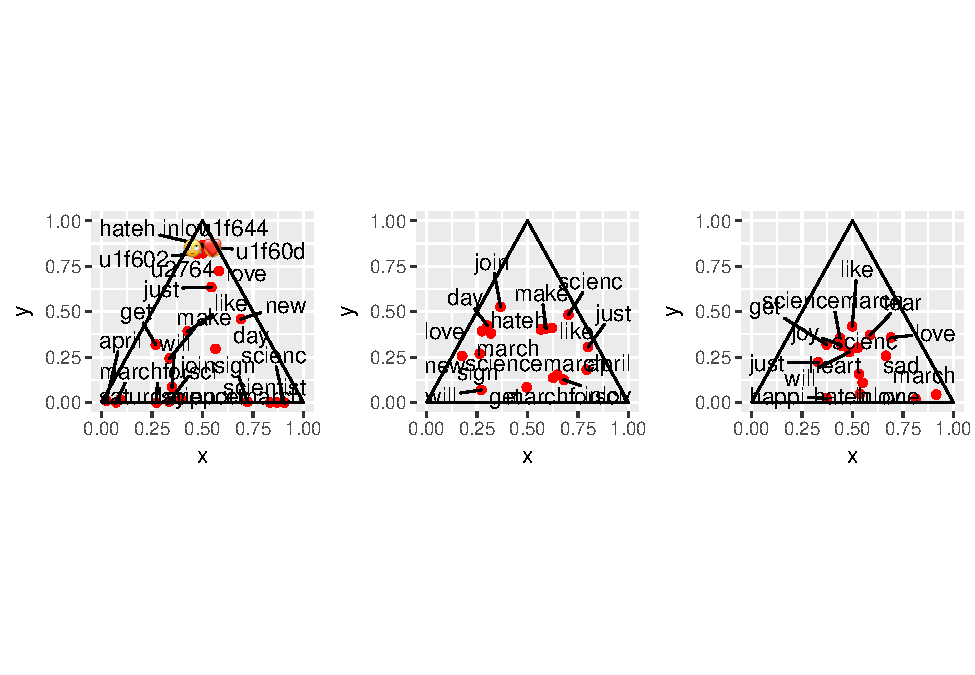
\includegraphics{CC_paper_files/figure-latex/unnamed-chunk-3-1.pdf}

\subsection{LDA on a raw data set}\label{lda-on-a-raw-data-set}

The first case was to run LDA on a raw data set. Different number of
topic dimensions were tested and the result of 3 topic dimension with 10
terms is provided in \autoref{tab:LDArawp}. The bar chart in
\autoref{fig:raw_bar} showed that LDA successfully distinguished the
corpus into three different topics. The bar chart illustrated that Topic
1 is related to `Science March', Topic 2 is related to `Hate her', and
Topic 3 is related to `Love her'. In order to visualize the probability
of a word given topic, a ternary plot was constructed in
\autoref{fig:raw_tern}. The ternary plot showed that four different
groups of words: three groups of words were strongly affiliated with one
of the topics. These groups of words were clustered at the end of each
vertices. The other group of words was located at the center of the
triangle which represented words that are not associated with a specific
topic. According to this ternary plot, emoji characters had strong
connection with a particular topic.

\begin{longtable}[]{@{}ccc@{}}
\caption{\label{tab:LDAraw} Output LDA with the raw data}\tabularnewline
\toprule
Topic 1 & Topic 2 & Topic 3\tabularnewline
\midrule
\endfirsthead
\toprule
Topic 1 & Topic 2 & Topic 3\tabularnewline
\midrule
\endhead
march & hateh & sciencemarch\tabularnewline
sciencemarch & inlov & scienc\tabularnewline
saturday & u1f60d & sign\tabularnewline
april & love & scientist\tabularnewline
will & just & will\tabularnewline
marchforsci & u2764 & join\tabularnewline
join & u1f602 & support\tabularnewline
get & get & marchforsci\tabularnewline
support & like & day\tabularnewline
make & u1f644 & new\tabularnewline
\bottomrule
\end{longtable}

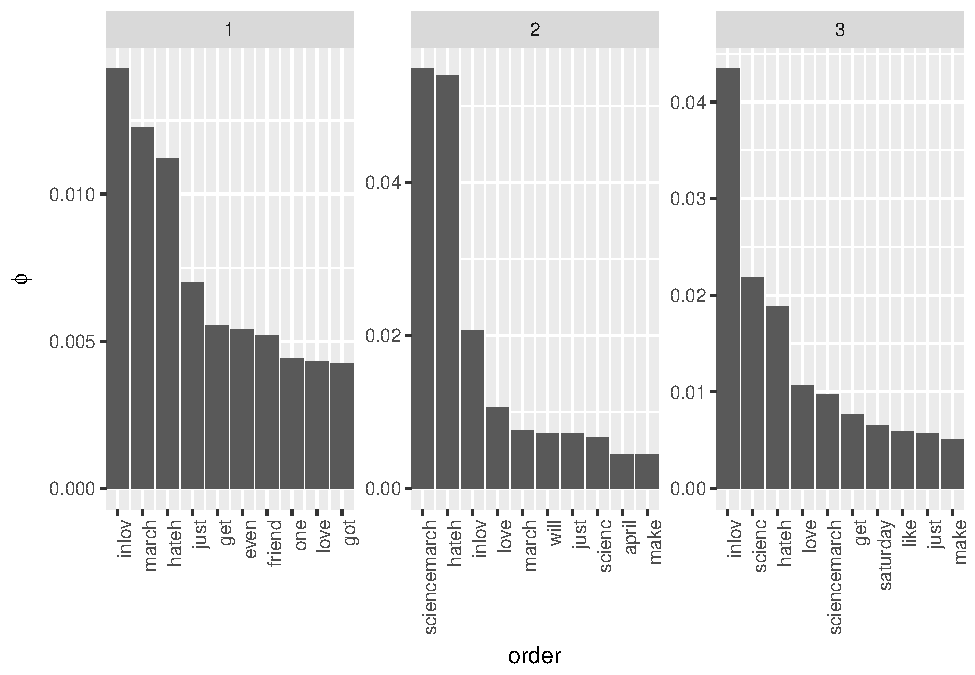
\includegraphics{CC_paper_files/figure-latex/unnamed-chunk-4-1.pdf}

\subsection{LDA without Unicode}\label{lda-without-unicode}

In most text mining examples, LDA is performed after removing the
Unicode information. For the second case, Unicode characters were
removed from the raw text data set before performing LDA. The result of
the LDA with three topic dimensions is provided in
\autoref{tab:LDA_no_unip}. The bar-chart in \autoref{fig:no_bar}
demonstrated that the LDA method did not distinguish the three topics
well. Topic 1 turned out to be a mixture of `Hate Her' and `Science
March', Topic 2 had all three topics, and Topic 3 was associated with
`Hate Her' and `Love Her'. Ternary plot constructed in
\autoref{fig:no_tern} shows that the output from the LDA was located at
the center of the ternary plot. This indicates that words had weak
connection to any topic dimensions.

\begin{longtable}[]{@{}ccc@{}}
\caption{\label{tab:LDA_no_uni} Output of LDA with the raw data without
the Unicode}\tabularnewline
\toprule
Topic 1 & Topic 2 & Topic 3\tabularnewline
\midrule
\endfirsthead
\toprule
Topic 1 & Topic 2 & Topic 3\tabularnewline
\midrule
\endhead
sciencemarch & hateh & inlov\tabularnewline
hateh & scienc & sciencemarch\tabularnewline
inlov & sciencemarch & hateh\tabularnewline
love & love & scienc\tabularnewline
will & inlov & just\tabularnewline
\bottomrule
\end{longtable}

\begin{longtable}[]{@{}cccccc@{}}
\caption{\label{tab:LDA_no_unip} Word prob. given topic}\tabularnewline
\toprule
1.term & 1.phi & 2.term & 2.phi & 3.term & 3.phi\tabularnewline
\midrule
\endfirsthead
\toprule
1.term & 1.phi & 2.term & 2.phi & 3.term & 3.phi\tabularnewline
\midrule
\endhead
sciencemarch & 0.0221 & hateh & 0.0461 & inlov & 0.0469\tabularnewline
hateh & 0.0199 & scienc & 0.0178 & sciencemarch & 0.0468\tabularnewline
inlov & 0.0190 & sciencemarch & 0.0148 & hateh & 0.0330\tabularnewline
love & 0.0149 & love & 0.0135 & scienc & 0.0135\tabularnewline
will & 0.0112 & inlov & 0.0111 & just & 0.0114\tabularnewline
march & 0.0098 & march & 0.0094 & get & 0.0062\tabularnewline
get & 0.0063 & just & 0.0064 & april & 0.0052\tabularnewline
new & 0.0062 & like & 0.0059 & like & 0.0048\tabularnewline
sign & 0.0048 & join & 0.0059 & marchforsci & 0.0044\tabularnewline
day & 0.0044 & make & 0.0053 & make & 0.0040\tabularnewline
\bottomrule
\end{longtable}

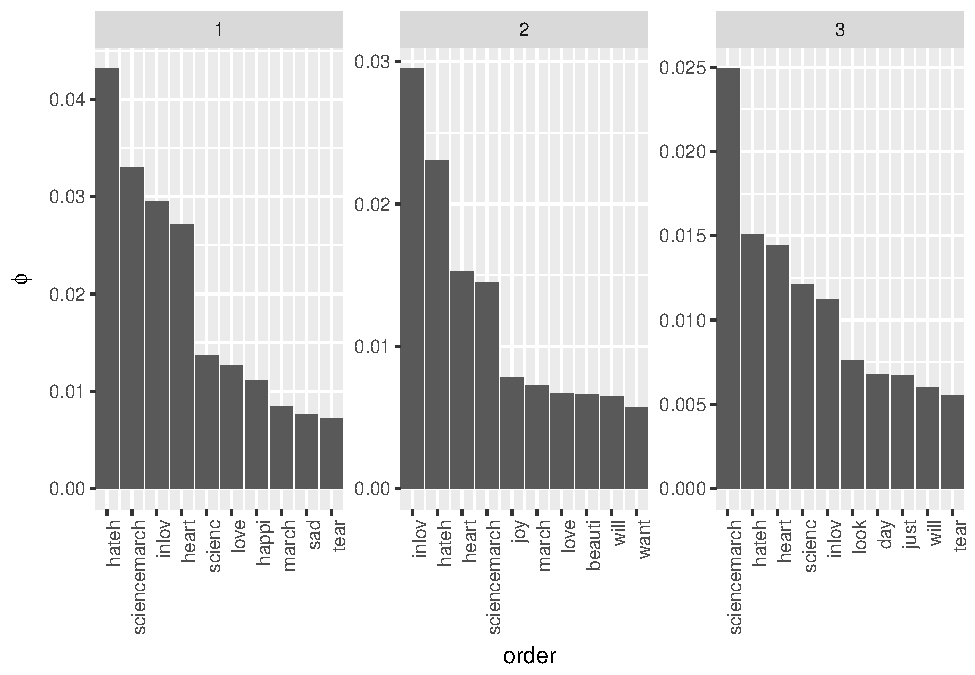
\includegraphics{CC_paper_files/figure-latex/unnamed-chunk-5-1.pdf}

\subsection{LDA with name translated}\label{lda-with-name-translated}

The last case was to perform LDA after translating the Unicode emoji
characters in English. The output of LDA with translation is provided in
\autoref{tab:LDA_tp}. The bar-chart in \autoref{fig:trans_bar} revealed
that the performance of the LDA method was ineffective. Words from `Hate
Her' and `Science March' were assigned to Topic 1, top words in Topic 2
were from `Love Her', `Hate Her', and `Science March', and top words in
Topic 3 were composed with words from `Hate Her' and `Love Her'. The
ternary plot in \autoref{fig:trans_tern} also showed that there were no
strong relationship between the words and a specific topic.

\begin{longtable}[]{@{}ccc@{}}
\caption{\label{tab:LDA_t} Output of LDA with translated
Unicode}\tabularnewline
\toprule
Topic 1 & Topic 2 & Topic 3\tabularnewline
\midrule
\endfirsthead
\toprule
Topic 1 & Topic 2 & Topic 3\tabularnewline
\midrule
\endhead
hateh & sciencemarch & hateh\tabularnewline
sciencemarch & scienc & inlov\tabularnewline
inlov & love & heart\tabularnewline
heart & heart & sciencemarch\tabularnewline
happi & inlov & march\tabularnewline
\bottomrule
\end{longtable}

\begin{longtable}[]{@{}cccccc@{}}
\caption{\label{tab:LDA_Tp} Word prob. given topic}\tabularnewline
\toprule
1.term & 1.phi & 2.term & 2.phi & 3.term & 3.phi\tabularnewline
\midrule
\endfirsthead
\toprule
1.term & 1.phi & 2.term & 2.phi & 3.term & 3.phi\tabularnewline
\midrule
\endhead
hateh & 0.0363 & sciencemarch & 0.0340 & hateh & 0.0424\tabularnewline
sciencemarch & 0.0294 & scienc & 0.0108 & inlov & 0.0337\tabularnewline
inlov & 0.0267 & love & 0.0107 & heart & 0.0260\tabularnewline
heart & 0.0221 & heart & 0.0106 & sciencemarch & 0.0191\tabularnewline
happi & 0.0098 & inlov & 0.0086 & march & 0.0146\tabularnewline
just & 0.0095 & tear & 0.0073 & love & 0.0126\tabularnewline
scienc & 0.0093 & like & 0.0062 & scienc & 0.0109\tabularnewline
joy & 0.0059 & joy & 0.0057 & sad & 0.0074\tabularnewline
get & 0.0059 & get & 0.0049 & tear & 0.0063\tabularnewline
will & 0.0052 & will & 0.0047 & one & 0.0060\tabularnewline
\bottomrule
\end{longtable}

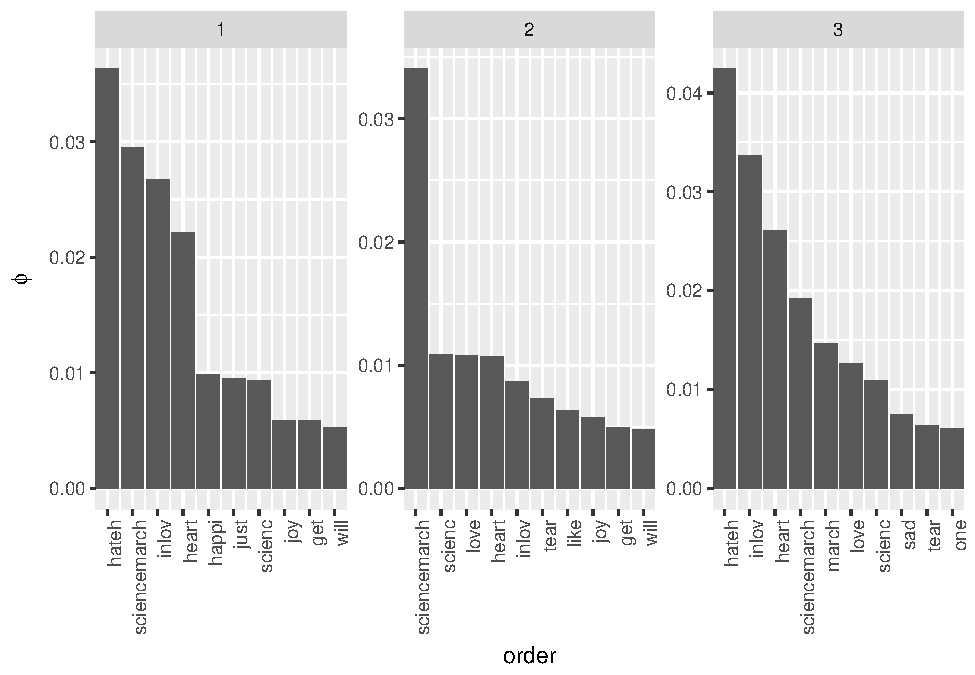
\includegraphics{CC_paper_files/figure-latex/unnamed-chunk-6-1.pdf}

\subsection{Discussion}\label{discussion}

The results of LDA outputs showed that LDA performed the best with emoji
information embedded as raw Unicode characters. The method well
distinguished the words assigned to three topics as shown in
\autoref{fig:raw_bar}, \autoref{fig:no_bar}, and
\autoref{fig:trans_bar}. The ternary plot in \autoref{fig:raw_tern},
\autoref{fig:no_tern}, and \autoref{fig:trans_tern} also supported the
claim by illustrating the strength of the relationship between a word
and the three topics. Emoji are rich in information, thus deleting the
entire character led to great information loss and consequently affected
the output of the LDA in case two.

Moreover, emoji characters aggregates- otherwise separated- n-gram words
into a single character. For example, commonly used Unicode characters
in the data set such as `U+1F602', `U+1F644', `U+1F60D', `U+1F618',
`U+2764', and `U+1F495' can be translated to English as `face with tears
of joy', `face with rolling eyes', `smiling face with heart eyes', `face
blowing a kiss', `red heart', and `two hearts' respectively. Although
the meaning of each emoji characters are different, their multi-gram
translations share words such as `face', and `heart'. Also, it produces
a few meaningless as a byproduct of translation. Since LDA methods are
affected by the frequency of words in the data set, the effect of the
translation method as alluded to above may affect the performance of the
LDA as shown in case three.

\section{Conclusion}\label{conclusion}

As the result of the exploratory analysis indicates,
user-generated-contents may contain Unicode emoji characters. These
emoji characters sometimes carry mixture of condensed information that
is difficult to express in words. The result of the output from the LDA
indicates that words such as ``heart'' that would have been neglected
using the traditional method may be saved when the Unicode characters
are translated into meanings.

\section{Appendix}\label{appendix}

\section{\texorpdfstring{\texttt{emoji} package in
R}{emoji package in R}}\label{emoji-package-in-r}

\textbf{Plan to change this part after posting the emoji package on CRAN}

\subsection{Description of the emoji
package}\label{description-of-the-emoji-package}

The \texttt{emoji} package contains information of the emoji v5.0 from
its official publisher the
\href{http://unicode.org/emoji/charts/emoji-list.html}{Unicode Consortium}.
The illustration of the web page is shown in \autoref{fig:uni_web}.

\begin{figure}[htbp]
\centering
\includegraphics[width=100mm]{"images/unicode_webpage".png}
\caption{Glimpse of the table of emoji on the Unicode.org website \label{fig:uni_web}}
\end{figure}

The data set \texttt{emoji} in the \texttt{emoji} package contains 8
variables:

uni\_no: Official number of emojis\(\\\) uni\_code: Formal Unicode of
emojis\(\\\) uni\_name: Official name of emojis\(\\\) cat1: Official
category of emojis\(\\\) cat2: Official sub-category of emojis from
cat1\(\\\) cat3: Official sub-category of emojis from cat2\(\\\)
uni\_keyws: Official keyword(s) of emojis\(\\\) uni\_png: Image of
emojis in PNG format represented in a matrix format\(\\\)

The package has a function \texttt{emoji\_info\_table} that summarizes
all emoji and their information used in a single character string.

\subsection{Scoring of Sentiment}\label{scoring-of-sentiment}

The characteristic of emoji (effectively delivers feelings and moods),
naturally leads text mining with emoji to sentiment analysis.
\texttt{tidytext} package in R has three general purpose lexicon sets.
The \texttt{AFINN} score words from -5 to 5 scale, \texttt{bing} assigns
words in binary category(positive and negative), and \texttt{nrc}assigns
words with more categories.

\section{More work}\label{more-work}

\begin{enumerate}
\def\labelenumi{\arabic{enumi}.}
\setcounter{enumi}{-1}
\tightlist
\item
  Technical details The \texttt{tm}, \texttt{topicmodels},
  \texttt{emoji}, \texttt{tidytext}, and \texttt{tidyverse} package in
  \texttt{R} was written to help the above analysis.
\item
  Check Stemming - scienc vs.~science
\item
  Check output again. Also, a check aggregation of short messages to
  avoid data sparsity.
\item
  LDA explanation
\item
  Description of the emoji package
\end{enumerate}


\end{document}
